% +++++++++++++++++++++++++++++++++++++++++++++++++++++++++++
% University of Southern Maine
% Department of Computer Science
% Discrete Mathematics II (COS 280)
% James Quinlan (https://cs.usm.maine.edu/~james.quinlan/)
% Homework Template
% +++++++++++++++++++++++++++++++++++++++++++++++++++++++++++

% EDIT Lines: 11, 12, 13
\def\filename{Simulated Annealing}   		   % included file (edit file)
\def\chapsec{Evolutionary Computing}  % Chapter/Section/Topic
\def\yourname{Simulated Annealing}	   % Your name
\def\course{COS 485}		   % Course (if different)

% ---------------- Do NOT Edit Below ------------------------
% -----------------------------------------------------------
\documentclass[11pt]{article}

\def\pf{\textit{Proof}: }

\usepackage{mathtools}
\usepackage{epsfig}
\usepackage{amsfonts}
\usepackage{amssymb}
\usepackage{amstext}
\usepackage{amscd}
\usepackage{amsmath}
\usepackage{xspace}
\usepackage{theorem}
\usepackage{float}
\usepackage[table]{xcolor}
\usepackage{color}
\usepackage{soul}
\usepackage{booktabs}
\usepackage{outlines}
\usepackage{enumitem}
\usepackage{algorithm}
\usepackage{algpseudocode}
\usepackage{pgf-pie}
\setenumerate[1]{label=\arabic*.}
\setenumerate[2]{label=(\alph*).}
\setenumerate[3]{label=\roman*.}
\setenumerate[4]{label=\alph*.}

\usepackage{hyperref}
\hypersetup{
    colorlinks=true,
    linkcolor=blue,
    filecolor=magenta,      
    urlcolor=cyan,
    pdftitle={\filename},
    pdfpagemode=FullScreen,
    }

% TikZ
\usepackage{tikz}
\usepackage{pgfplots}
\pgfplotsset{compat=1.15}
\usepackage{mathrsfs}
\usetikzlibrary{arrows}

% Colors
\definecolor{stainlessSteel}{cmyk}{0,0,0.02,0.12}

% Document Geometry
\makeatletter
 \setlength{\textwidth}{6.75in}
 \setlength{\oddsidemargin}{0in}
 \setlength{\evensidemargin}{0in}
 \setlength{\topmargin}{0.0125in}
 \setlength{\textheight}{9.0in}
 \setlength{\headheight}{0pt}
 \setlength{\headsep}{0pt}
 \setlength{\marginparwidth}{59pt}

 \setlength{\parindent}{0pt}
 \setlength{\parskip}{5pt plus 1pt}
 \setlength{\theorempreskipamount}{5pt plus 1pt}
 \setlength{\theorempostskipamount}{0pt}
 \setlength{\abovedisplayskip}{8pt plus 3pt minus 6pt}
 \setlength{\intextsep}{15pt plus 3pt minus 6pt}

 % Headings
 \renewcommand{\section}{\@startsection{section}{1}{0mm}%
    {2ex plus -1ex minus -.2ex}%
    {1.3ex plus .2ex}%
    {\normalfont\Large\bfseries}}%
 \renewcommand{\subsection}{\@startsection{subsection}{2}{0mm}%
    {1ex plus -1ex minus -.2ex}%
    {1ex plus .2ex}%
    {\normalfont\large\bfseries}}%
 \renewcommand{\subsubsection}{\@startsection{subsubsection}{3}{0mm}%
    {1ex plus -1ex minus -.2ex}%
    {1ex plus .2ex}%
    {\normalfont\normalsize\bfseries}}
 \renewcommand\paragraph{\@startsection{paragraph}{4}{0mm}%
    {1ex \@plus1ex \@minus.2ex}%
    {-1em}%
    {\normalfont\normalsize\bfseries}}
 \renewcommand\subparagraph{\@startsection{subparagraph}{5}{\parindent}%
    {2.0ex \@plus1ex \@minus .2ex}%
    {-1em}%
    {\normalfont\normalsize\bfseries}}
\makeatother

\newcounter{thelecture}

\newenvironment{proof}{{\bf Proof:  }}{\hfill\rule{2mm}{2mm}}
\newenvironment{proofof}[1]{{\bf Proof of #1:  }}{\hfill\rule{2mm}{2mm}}
\newenvironment{proofofnobox}[1]{{\bf#1:  }}{}
\newenvironment{example}{{\bf Example: }}{\hfill\rule{0mm}{0mm}} % change 2mm 2mm for square

%\renewcommand{\theequation}{\thesection.\arabic{equation}}
%\renewcommand{\thefigure}{\thesection.\arabic{figure}}

\newtheorem{fact}{Fact}
\newtheorem{lemma}[fact]{Lemma}
\newtheorem{theorem}[fact]{Theorem}
\newtheorem{definition}[fact]{Definition}
\newtheorem{corollary}[fact]{Corollary}
\newtheorem{proposition}[fact]{Proposition}
\newtheorem{claim}[fact]{Claim}
\newtheorem{exercise}[fact]{Exercise}

% math notation
\newcommand{\R}{\ensuremath{\mathbb R}}
\newcommand{\Z}{\ensuremath{\mathbb Z}}
\newcommand{\N}{\ensuremath{\mathbb N}}
\newcommand{\B}{\ensuremath{\mathbb B}}
\newcommand{\F}{\ensuremath{\mathcal F}}
\newcommand{\SymGrp}{\ensuremath{\mathfrak S}}
\newcommand{\prob}[1]{\ensuremath{\text{{\bf Pr}$\left[#1\right]$}}}
\newcommand{\expct}[1]{\ensuremath{\text{{\bf E}$\left[#1\right]$}}}
\newcommand{\size}[1]{\ensuremath{\left|#1\right|}}
\newcommand{\ceil}[1]{\ensuremath{\left\lceil#1\right\rceil}}
\newcommand{\floor}[1]{\ensuremath{\left\lfloor#1\right\rfloor}}
\newcommand{\ang}[1]{\ensuremath{\langle{#1}\rangle}}
\newcommand{\poly}{\operatorname{poly}}
\newcommand{\polylog}{\operatorname{polylog}}

% Anupam's abbreviations
\newcommand{\e}{\epsilon}
\newcommand{\half}{\ensuremath{\frac{1}{2}}}
\newcommand{\junk}[1]{}
\newcommand{\sse}{\subseteq}
\newcommand{\union}{\cup}
\newcommand{\meet}{\wedge}
\newcommand{\dist}[1]{\|{#1}\|_{\text{dist}}}
\newcommand{\hooklongrightarrow}{\lhook\joinrel\longrightarrow}
\newcommand{\embeds}[1]{\;\lhook\joinrel\xrightarrow{#1}\;}
\newcommand{\mnote}[1]{\normalmarginpar \marginpar{\tiny #1}}


% -----------------------------------------------------------
% Header
\newcommand{\hwheadings}[3]{
{\chapsec } \hfill {{ \yourname }} \hfill {{ \course #1}}\\
{{\bf } #2} \hfill { #3} 
\rule[0.051in]{\textwidth}{0.0025in}
%\thispagestyle{empty}
}

% Document begins here 
\begin{document}
\hwheadings{}{}{}

\section*{\centering Simulated Annealing}

\section*{Background Information}%
\label{sec:background}

\subsection*{What is \textit{Annealing}?}%
\label{sub:annealing}

Annealing is the process of heating a material to a specific temperature to make it easier to work with
(Materials like glass, steel, copper, etc). After being heated to a high temperature, the cooling
of the material is controlled to allow the material to be reshaped and harden with its new shape.

With \textit{Simulated} Annealing, think of our solution canidate as the glass or metal material. 
At first, the termperature is very high and the solution is very malleable and seceptible to change,
whether it be a good or bad change. But as time goes on, it gets harder to change the solution 
because it cools. \textit{`Changing'} the solution is taking a worse solution, in the context of Simulated Annealing.

\subsection*{Purpose}%
\label{sub:purpose}

The purpose of using a Simulated Annealing algorithm is \textit{optimization}. There are
many problems that take a factorial amount of time to come up with an optimal solution. With
simulated annealing, we can take educated guesses to find a very good solution in polynomial time.

Another reason Simulated Annealing is used is the \textit{Hill Climbing Problem}, or to prevent
your solutions from getting stuck in a \textit{local maxima} or \textit{local minima}.

\begin{center}
  \label{fig:example-function}
  Example function to optimize

  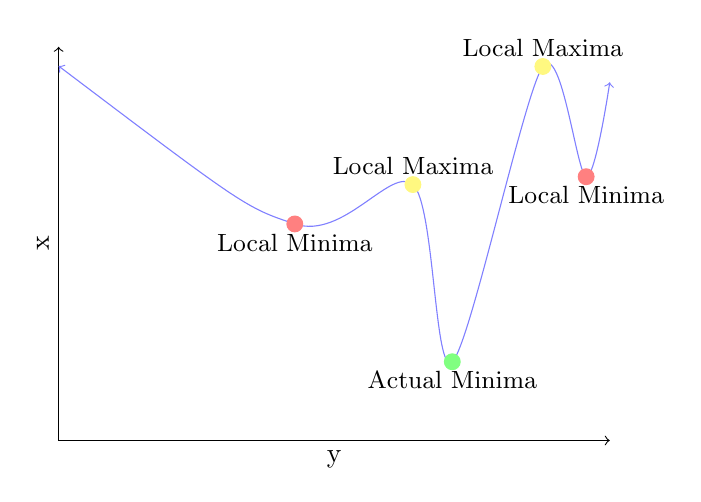
\begin{tikzpicture}
  \coordinate (bottom) at (5,1);
  \coordinate (lmen) at (3 , 2.75);
  \coordinate (lman) at (4.5 , 3.25);
  \coordinate (rmen) at (6.7,3.35);
  \coordinate (rman) at (6.15,4.75);
  \coordinate (lkant) at (0,4.756);
  \coordinate (rkant) at (7,4.55);
  \coordinate (o) at (0,0);
  \coordinate (x) at (7,0);
  \coordinate (y) at (0,5);
  \draw [<->] (y) -- node [rotate=90, above] {x} (o) -> node [below] {y} (x);
  \draw [blue!50,<->] plot [smooth] coordinates {(lkant) (lmen) (lman) (bottom) (rman) (rmen) (rkant)};
  \filldraw[color = green!50] (bottom) circle  (0.1) node [below,color=black] {\small Actual Minima};
  \filldraw [color = red!50] (lmen) circle (0.1) node [below,color=black] {\small Local Minima };
  \filldraw [color = red!50] (rmen) circle (0.1) node [below,color=black] {\small Local Minima};
  \filldraw [color = yellow!50] (lman) circle (0.1) node [above,color=black] {\small Local Maxima};
  \filldraw [color = yellow!50] (rman) circle (0.1) node [above,color=black] {\small Local Maxima};
  \end{tikzpicture}
\end{center}

\subsection*{Simulated Annealing Basics}%
\label{sub:basics}

A \textit{Cooling Function} is used to slowly decrease the Temperature for the algorithm.
As the temperature decreses, there is less chances of taking a worse solution.
In general, the probability will never be more than 50\% to take a worse solution, however it can be lower.
\[
  p = \frac{1}{1 + e^{\Delta E / T_k}} 
\]
A random number, $0 \le r \le  1$ should be generated, and if  $p \ge r$ then the new canidate solution
will be selected despite being a `worse' solution.

$\Delta E$ is the change in Energy. When simulating annealing, energy is how `good' a solution is
for the respective problem. In the example of the Traveling Salesman Problem, a lower energy would be
a lower total weight of all edges in the cycle.

\begin{center}
  Probability of Accepting a Worse Solution

  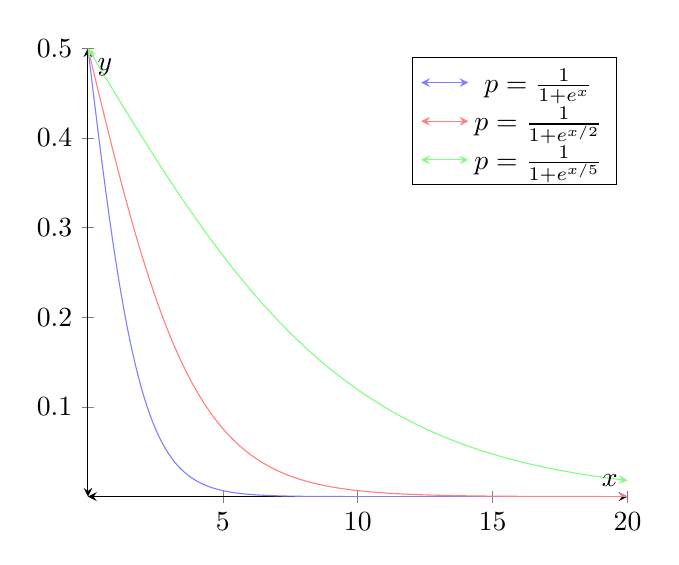
\begin{tikzpicture}[>=stealth]
    \label{fig:probability}
    \begin{axis}[
      xmin=0,xmax=20,
      ymin=0,ymax=0.5,
      axis x line=middle,
      axis y line=middle,
      axis line style=<->,
      xlabel={$x$},
      ylabel={$y$},
      legend entries={
        $p = \frac{1}{1 + e^{x}}$,
        $p = \frac{1}{1 + e^{x/2}}$,
        $p = \frac{1}{1 + e^{x/5}}$,
      },]
      \addplot[no marks,blue!50,<->] expression[domain=0:20,samples=1000]{1/(1+e^x)};
      \addplot[no marks,red!50,<->] expression[domain=0:20,samples=1000]{1/(1+e^(x/2))};
      \addplot[no marks,green!50,<->] expression[domain=0:20,samples=1000]{1/(1+e^(x/5))};
    \end{axis}
  \end{tikzpicture}
\end{center}

If the solution is marginally worse, and as the temperature decreases, there is a higher chance for $x$' to be 
a larger number, which lowers the chances of taking the worse solution.

The Temperature starts off very high, and lowers depending on the cooling algorithm. If the temperature
decreases too rapidly, or does not start at a high enough number, canidate solutions can get stuck in a local minima or maxima.

\begin{center}
  Temperature Threshold

  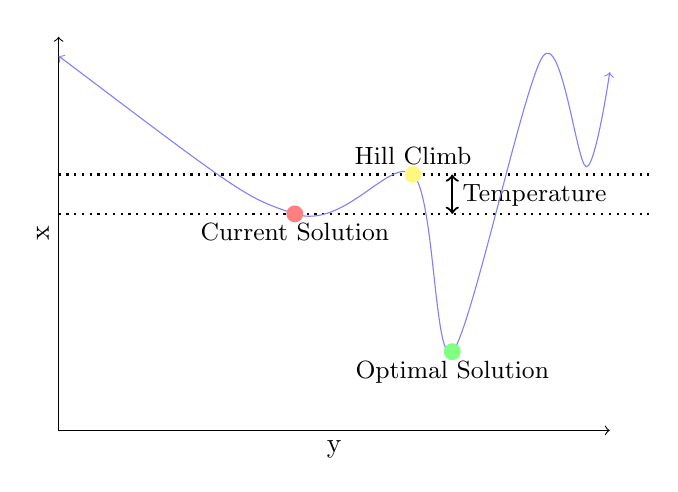
\begin{tikzpicture}
  \label{fig:threshold}
  \coordinate (bottom) at (5,1);
  \coordinate (lmen) at (3 , 2.75);
  \coordinate (lman) at (4.5 , 3.25);
  \coordinate (rmen) at (6.7,3.35);
  \coordinate (rman) at (6.15,4.75);
  \coordinate (lkant) at (0,4.756);
  \coordinate (rkant) at (7,4.55);
  \coordinate (o) at (0,0);
  \coordinate (x) at (7,0);
  \coordinate (y) at (0,5);
  \draw [thick, dotted] (0, 2.75) -- (7.5,2.75);
  \draw [thick, dotted] (0, 3.25) -- (7.5,3.25);
  \draw [<->] (y) -- node [rotate=90, above] {x} (o) -> node [below] {y} (x);
  \draw [black, thick, <->] (5,2.75) -- (5,3.25) node[below right]{\small Temperature};
  \draw [blue!50,<->] plot [smooth] coordinates {(lkant) (lmen) (lman) (bottom) (rman) (rmen) (rkant)};
  \filldraw[color = green!50] (bottom) circle  (0.1) node [below,color=black] {\small Optimal Solution};
  \filldraw [color = red!50] (lmen) circle (0.1) node [below,color=black] {\small Current Solution};
  \filldraw [color = yellow!50] (lman) circle (0.1) node [above,color=black] {\small Hill Climb};
  \end{tikzpicture}
\end{center}

\section*{General Simulated Annealing Algorithm}%
\label{sec:generic-algorithm}

\begin{algorithm}[H]
  \caption{Generic Simulated Annealing}
  \label{alg:simulated-annealing}
  \begin{algorithmic}
  \State \textbf{Note}: The goal is to \textit{Minimize} for this example.
  \State \textbf{Inputs}:
  \State $T_{0}$, Initial temperature
  \State $s_{0}$, Initial solution/state
  \State $E$, \textit{Energy} function
  \State $J$, \textit{Cooling} function
  \State $N$, \textit{Neighbor} function
  \Require $T_{0} > 1$
  \State $T \gets T_{0}$
  \State $s_{k} \gets s_{0}$
  \State $k \gets 0$
  \Repeat
  \State $s_{k+1} \gets N(s_{k})$ \Comment{Find a neighbor of the current solution}
  \State $\Delta E \gets E(s_{k+1}) - E(s_{k})$ 
  \If{$\Delta E < 0$} 
    \State $s_{k} \gets s_{k+1}$ \Comment{Accept the better solution}
  \ElsIf{$p \ge rand(0,1)$***}
    \State $s_{k} \gets s_{k+1}$ \Comment{Accept the worse solution}
  \Else
    \State $s_{k} \gets s_{k}$ \Comment{Keep the previous solution}
  \EndIf
  \State $T_{k} \gets J(T_{k})$ \Comment{The temperature cools}
  \State $k++$
  \Until{$T_{k} = 1$ or $s_{k}$ satisfies some condition}
  \end{algorithmic}
\end{algorithm}
\[
  \textrm{*** } p = \frac{1}{1 + e^{\Delta E / T_k}} \textrm{, probability of accepting the worse solution}
\] 
\end{document}
% -----------------------------------------------------------
